\documentclass[]{tp}
\titre{TP7 : Propagation d'ondes}  
\usetikzlibrary{positioning}
\begin{document}
%\small


\section{Corde de Melde}%
\label{sec:corde_de_melde}
La corde de Melde est une cordelette reliée d’un côté à une masse $m$ par l'intermédiaire d’une poulie, et de l’autre côté à un vibreur qui génère sur la corde des oscillations transversales de fréquence $f$. 

On note $L$ la longueur \emph{utile}  de la corde, c’est-à-dire la longueur de corde entre le vibreur et la poulie au repos.

On peut observer la corde sous un éclairage continu ou avec un stroboscope qui émet des flashs lumineux très brefs à une fréquence $f_s$ réglable. 

On repérera les positions longitudinales sur la corde par l’abscisse $x\in [0,L]$, l'origine se situant au niveau du vibreur ; et la position transversale de la corde par la cote $z$, l'origine se situant au niveau de la position au repos.

\begin{center}
  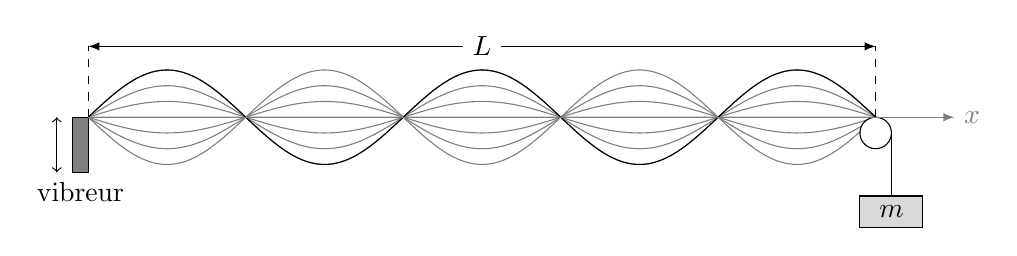
\begin{tikzpicture}
    \draw[fill=gray] (-0.2,-0.7) rectangle (0, 0);
    \draw[<->] (-0.4, -0.7) -- (-0.4, 0);
    \draw (-0.1, -0.7) node[below] {vibreur};
    \foreach \a in {-0.6,-0.4,...,0.61}{
      \draw[gray] plot[domain=0:10, samples=200] (\x, {\a*sin(360*\x/4) });
    }
    \draw[] plot[domain=0:10, samples=200] (\x, {0.6*sin(360*\x/4) });
  \draw[fill=white] (10,-0.2) circle(0.2);
  \draw (10.2, -0.2) -- ++(0,-0.8);
  \draw[fill=gray!30] (9.8, -1) rectangle (10.6, -1.4);
  \draw (10.2, -1.2) node {$m$}; 

  \draw[dashed] (0,0) -- ++(0,0.9) coordinate(A); 
  \draw[dashed] (10,0) -- ++(0,0.9) coordinate (B);
  \draw[latex-latex] (A) -- (B) node[midway, fill=white] {$L$}; 
  \draw[-latex,gray] (0,0) -- (11,0) node[right]{$x$};
  \end{tikzpicture}
\end{center}

\subsection{Propagation d'onde transversale sur la corde}%
\label{sub:propagation_d_onde_transversale_sur_la_corde}

L'oscillation générée par le vibreur à une extrémité de la corde se propage le long de celle-ci et \emph{rebondit} à l'extrémité fixe (poulie) de la corde. Elle revient ensuite vers le vibreur en sens inverse. La \emph{célérité} (vitesse) de propagation de l'oscillation est donnée par la relation : 
%
\[c = \sqrt{\frac{T}{\mu}}\] 
%
avec $c$ en \si{m/s}, $T$ la tension de la corde en N et $\mu$ la masse linéique (masse par unité de longueur) en \si{kg\per\meter}. Pour une corde donnée ($\mu$ fixée), la célérité ne dépend donc que de la tension $T$ imposée à la corde par la masse $m$.

Les oscillations imposées par le vibreur étant de faible amplitude par rapport à celle des oscillations de la corde, on considérera que la corde est immobile au niveau du vibreur.

Dans la plupart des cas, on n'observe rien de spécial sur la corde. Par contre, si la fréquence du vibreur permet que l'aller-retour se fasse dans une durée telle que les conditions aux limites sont respectées (immobilité en $x=L$ et en $x=0$), l'oscillation peut se conserver et s'amplifier : on parle de \emph{résonance}. La superposition de toutes ces \emph{ondes progressives} génère alors ce qu'on appelle une \emph{onde stationnaire} : certains points de la corde ne bougent plus (\emph{n\oe{}uds de vibration}), d'autres ont une amplitude de vibration maximale (\emph{ventres de vibration}). La corde prend l'allure d'une sinusoïde : à une date $t$, 
%
\[z(x,t) = z_0\cos\left(2\pi f t\right) \cos\left(\frac{2\pi}{\lambda} x + \varphi \right).\] 
%
$\lambda$ est la \emph{longueur d'onde} des vibrations, c'est-à-dire leur période spatiale.

Lorsque la fréquence de vibration est suffisamment élevée, la persistance rétinienne fait qu'on voit des fuseaux sur la corde, comme représenté sur la figure ci-dessus.

\begin{itemize}
  \item Écrire les deux équations correspondant aux conditions aux limites. En déduire $\varphi$, ainsi que la relation existant entre $\lambda$ et $L$ (cette relation fait intervenir un entier $n$).

  \item Sachant que $\lambda = \frac{c}{f}$, expliquer pourquoi à $m$, $\mu$ et $f$ fixées, seule la longueur $L$ de la corde va jouer sur l'établissement ou non d'ondes stationnaires.

  \item Pour $n = 4$, représenter l'allure de la corde à une date $t$ quelconque. Combien y a-t-il de n\oe{}uds ? de ventres ? Généraliser pour $n$ quelconque.

\end{itemize}


\subsubsection{Manipulation}%
\label{ssub:manipulation}
On utilisera une masse de \SI{200}{g} et une longueur de corde de l'ordre de \SI{1}{m}. 

\begin{itemize}
  \item Ajuster la longueur utile $L$ de la corde et noter les longueurs de la corde pour lesquelles on obtient des ondes stationnaires. On notera pour chaque longueur le nombre de ventres de vibration observés.
\end{itemize}


On souhaite mesurer la fréquence de vibration par stroboscopie. Pour cela on utilise un stroboscope qui produit des flashs lumineux très brefs à une fréquence bien définie.

\begin{itemize}
  \item Brancher le stroboscope sur la sortie \texttt{OUTPUT \SI{50}{\ohm}} du GBF. Sélectionner un signal carré, tirer sur le bouton \texttt{SYMETRY} et le tourner au maximum vers la gauche. Mettre le \texttt{LEVEL} au maximum. Le stroboscope émet des flashs à la fréquence $f_s$ indiquée par le GBF. 
\end{itemize}

Pour déterminer la fréquence $f$ d'oscillation de la corde, il faut déterminer la fréquence $f_s$ du stroboscope la plus haute possible qui permet de ne voir qu'une seule corde qui semble immobile. 

\begin{itemize}
  \item Déterminer la fréquence d'oscillation de la corde
  \item Que se passe-t-il si on éclaire la corde avec une fréquence $f=\frac{f_s}{2}$ ?
  \item Que se passe-t-il si on éclaire la corde avec une fréquence légèrement supérieure ou légèrement inférieure à $f$ ? 

  \item Déterminer la longueur d'onde de l'onde qui se propage sur la corde et en déduire la célérité de l'onde ainsi que la masse linéique de la corde.
\end{itemize}




\section{Propagation d'ultrasons}
Le but de cette partie est de générer une onde ultra-sonore à l'aide d'un émetteur puis de visualiser l'onde reçue par un récepteur sur un oscilloscope. On mesurera la longueur d'onde et la célérité de l'onde émise.
  \begin{center}
  \begin{tikzpicture}[scale=1, transform shape]
    \draw (0,0) node[draw, rectangle, minimum width=2cm, minimum height=1cm] (Alim) {Alimentation};   

    \node[draw, inner sep=3mm] (emetteur) [right=1cm of  Alim] {Émetteur};    
    \node[draw, inner sep=3mm] (recepteur) [right=4cm of  emetteur] {Récepteur};    
    \node[draw, inner sep=6mm] (oscillo) [right=1cm of  recepteur] {Oscilloscope};    
    \draw (Alim) -- (emetteur);
    \draw (emetteur.south) -- ++(0,-0.5) -| ($(oscillo.south)+(-0.5, 0)$) coordinate(CH1) node[above]{CH1};
    \draw (recepteur.south) -- ++(0,-0.8) -| ($(oscillo.south)+(+0.5, 0)$) coordinate(CH2) node[above]{CH2};
    \fill (CH1) circle(2pt);
    \fill (CH2) circle(2pt);
    \draw[latex-latex] (emetteur.east) -- (recepteur.west) node[midway, fill=white]{$d$}; 

  \end{tikzpicture}
  \end{center}
 
\subsection{Émission d'impulsions}
\begin{itemize}
  \item Utiliser les émetteurs en mode \emph{impulsion} pour déterminer la célérité du son dans l'air.
\end{itemize}
 On peut obtenir une valeur de la vitesse du son dans l'air à la température $T$ (en degrés celsius entre -20 et \SI{+40}{\celsius}) avec une erreur inférieure à \SI{0.2}{\percent} avec la formule approchée :
    \begin{equation*}
      c=(331.5+0.607\cdot T)~\si{\m\per\s}
    \end{equation*}
\begin{itemize}
  \item La valeur calculée est-elle compatible avec celle que vous avez mesurée ?
\end{itemize}


\subsection{Émission en continu}
On règle l'émetteur pour qu'il émette une onde en continu.
\begin{itemize}
  \item Mesurer à l'oscilloscope la période $T$ du signal émis, en déduire la valeur de la fréquence $f$. 

  \item Déterminer la longueur d'onde de l'onde émise en repérant les positions du récepteur pour lesquelles les ondes émises et reçues sont en phase.

  \item Vérifier la relation entre $c$, $f$, et $\lambda$. 
\end{itemize}




\end{document}
